%%%%%% Computing Chapter  %%%%%%%%%%%%%%%%
 
\chapter{Computing Frontier: Distributed Computing and Facility Infrastructures}
\label{chap:mag}


%%%%%%%%%%%%%%%%%%%%%%%%%%%%%%%%%%%%%%%%%%%%%%%%%%%%%%%%%%%
%%%%%%%%%%%%%%%%%%%%%%%%%%%%%%%%%%%%%%%%%%%%%%%%%%%%%%%%%%%
%%%%%%%%%%%%%%%%%%%%%%%%%%%%%%%%%%%%%%%%%%%%%%%%%%%%%%%%%%%
%%%%%%%%%%%%%%%%%%%%%%%%%%%%%%%%%%%%%%%%%%%%%%%%%%%%%%%%%%%
\begin{center}\begin{boldmath}

\input CpF-I2/authorlist.tex
%Conveners are also listed separately in authorlist.tex

\end{boldmath}\end{center}

%%%%%%%%%%%%%%%%%%%%%%%%%%%%%%%%%%%%%%%%%%%%%%%%%%%%%%%%%%%
%%%%%%%%%%%%%%%%%%%%%%%%%%%%%%%%%%%%%%%%%%%%%%%%%%%%%%%%%%%
%%%%%%%%%%%%%%%%%%%%%%%%%%%%%%%%%%%%%%%%%%%%%%%%%%%%%%%%%%%
%%%%%%%%%%%%%%%%%%%%%%%%%%%%%%%%%%%%%%%%%%%%%%%%%%%%%%%%%%%

\section{Introduction}
\label{sec:comp-intro}

The field of particle physics has become increasingly reliant on large-scale computing resources to address the challenges of analyzing large datasets, completing specialized computations and simulations, and allowing for wide-spread participation of large groups of researchers.  For a variety of reasons, these resources have become more distributed over a large geographic area, and some resources are highly specialized computing machines.  In this report for the Snowmass Computing Frontier Study, we consider several questions about distributed computing and facility infrastructures that could impact future resource requirements and research directions.

\section{Current HEP Use of the U.S. National Computing Infrastructure}

Different computational problems in particle physics are naturally suited for different kinds of computing facilities.  In general, there are two paradigms.  One is high-throughput computing (HTC), which is implemented in standard commodity computers and can address problems that are “embarrassingly parallel,” i.e., those that can be computed independently with the results combined afterward.  The other is high performance computing (HPC), which uses supercomputers to solve large problems by distributing computational work among many processors and using specialized high-speed, low-latency networks to communicate partial results among processors during execution of the job.

The Worldwide LHC Computing Grid (WLCG) is an HTC resource that is the main computational resource used by the LHC experiments, of which ATLAS and CMS have the largest computing needs.  As the name implies, the WLCG is an example of a grid infrastructure, which is described in much more detail in Section XXX [needs proper LaTeX reference to grid section].  There are over 170 facilities connected to the WLCG, distributed over 36 countries.  Fifteen of those sites are located in the United States, and they tend to have more resources than the average WLCG site.  The WLCG is organized into a tiered hierarchy of sites, in which sites at each tier have different computational responsibilities and service levels, and thus different hardware configurations.  The Tier-0 center is at CERN; it is responsible for prompt reconstruction of detector data, some calibration and alignment tasks and keeping a custodial copy of the raw data.  There are currently twelve Tier-1 sites, which keep a second custodial copy of the raw data, reprocess older data with improved calibration and alignment constants, perform skims of large data samples, and archive simulated datasets.  Both Tier-0 and Tier-1 centers operate tape libraries and have 24/7 system support.  The remaining sites are Tier-2 sites, which host data samples for physics analysis and generate simulated datasets.  Tier-2 centers typically only have business-hours support within their time zone.  The facilities are composed of large clusters of commodity machines powered by x86-style processors, which are accessed through batch scheduling systems.

The computational problems of the LHC experiments are well matched to the structure of the WLCG.  Computations are centered around individual, statistically independent collision events, and this “embarrassingly parallel” regime works well for the HTC systems that the WLCG provides.  This scheme has served the LHC experiments very well.  The current resources of the WLCG are 2 MHS06 of CPU and 190 PB of disk.  CMS and ATLAS used about 300,000 cores continuously during 2012, resulting in about 2.6 billion CPU hours.  These resources, along with robust middleware and a strong effort in operations, have allowed the experiments to turn around physics results very quickly.  The workflows for the experiments, be they for data processing, calibration, simulation or user analysis, have performed as expected, and any concerns about scaling with the expected increase in resources should be able to be addressed in the course of normal operations.  There is a good window for this work during the current LHC shutdown.

As discussed below, whether the WLCG will continue to serve the needs of the LHC experiments depends very much on how WLCG capacity evolves, and how efficiently the experiments can make use of it.  This is an important question, given the anticipated growth in LHC luminosity (from $7 x 10^33$ to $1 x 10^34 /cm^2/s$), event complexity due to pileup (from a typical 20 extra interactions per event in the previous LHC run to 25 in the 2015 run), and trigger rate to maintain sensitivity to the Higgs boson and new-physics signatures (from 300 Hz to perhaps 1 kHz).  However, any changes to the WLCG usage can be made in an evolutionary fashion, and the underlying paradigm of HTC should continue to work.

Because of the sheer scale of the existing WLCG resources, we anticipate that the WLCG will remain the main resource for LHC experiment computations.  However, the use of other facilities, such as those described below, should be explored to see if they can successfully perform the same computations and thus augment the LHC computing capacity.

National High Performance Computing centers are used and required by a number of HEP projects, including
\begin{itemize}
\item Lattice QCD (Energy)
\item Accelerator design and R\&D (Energy and Intensity)
\item Data analysis and synthetic maps (Cosmic)
\item N-body and hydro cosmology simulations (Cosmic)
\item Supernova modeling (Cosmic)
\end{itemize}

A great need for HPC computing, driven by the needs of LQCD and computational cosmology but required by other fields as well, will outpace even the historical trend (see Figure \ref{fig:NERSC-Computational-Hours}), even as extrapolation of those trends becomes uncertain due to power and technology limitations.

\begin{figure}[p]
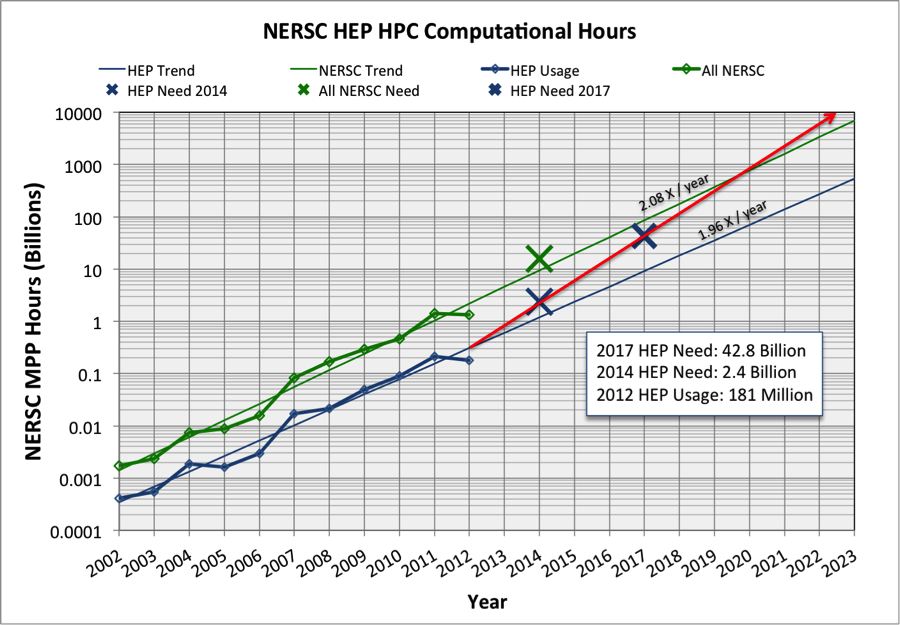
\includegraphics[width=\textwidth]{CpF-I2/images/2013-NERSC-Usage-HEP.pdf}
\caption{Historical normalized computing hours used at NERSC (green line) and just for HEP projects (blue line). Results from NERSC requirements reviews with HEP scientists and DOE program managers (large blue crosses) show a need for computing greater than what will be supplied by extrapolating the trend.}
\label{fig:NERSC-Computational-Hours}
\end{figure}

Intensity Frontier experiments have combined computing requirements
on a scale that could map onto the HPC center model. The experiments 
have a diverse set of needs, but a survey found that
there is significant commonality among them. Some
experiments have already made effective use of HPC centers' facilities and
expertise. For example, the Daya Bay experiment analysis was conducted at NERSC, which also served as the Tier 1 data center. 
NERSC also has expertise gained from supporting KAMLAND, IceCube, BaBar, SNO, ALICE, ATLAS, and Palomar PTF data analysis. 
There may be an opportunity for Intensity Frontier experiment to band together and take advantage of centralized facilities
as a source of computing and storage and a gathering place for software repositories and expertise on common requirements.

One effort, Perturbative QCD,  that has largely relied on HTC computing to date has already started using HPC centers and expects to 
expand those efforts to be able to complete the calculation of important background and signal reactions at the
LHC.  
They have determined that it would be beneficial to make the national HPC
facilities ALCF~\cite{ALCF}, OLCF~\cite{OLCF} and NERSC~\cite{NERSC}
generally accessible to particle theorists and
experimentalists in order to enable the use of existing
calculational tools for experimental studies involving extensive
multiple runs without depending on the computer power and manpower
available to the code authors. Access to these facilities will also
allow prototyping the next generation of parallel computer programs
for QCD phenomenology and precision calculations.

 
\section{Future Availability of Resources}


The needed computing resources for Energy Frontier experiments are currently set by the needs of the CMS and ATLAS experiments.  Both of these experiments have had several years of running experience and have developed the tools to predict future resource needs as a function of experimental parameters such as the trigger rate, pileup distribution, event size, number of reprocessing and analysis passes per year and so forth.  These models have been shown to be reasonably predictive.  [Ref a CHEP paper on this?]

It currently appears that the needs will be met for the foreseeable (~10 year) future as long as several conditions are satisfied.  So far, the funding for the WLCG has been roughly constant, allowing resource growth to continue with Moore’s Law.  Experiments have been able to adjust their computing models to adapt to the available growth in resources along with the growth in data sets.  While Moore’s Law does not seem to hold as well as it used to, resources should still grow over time, although not as quickly as before.  Near-constant WLCG funding will be necessary for the experiments to keep up with growing datasets and event complexity.  

Meanwhile, computing architectures are changing, and the experiments’ software bases must evolve to keep up with them.  Adapting the software to take advantage of manycore and multicore 
processor architectures is also critical for LHC experiments to meet their computing needs.  The experiments will also need to find greater efficiencies in resource usage, for both processing and disk resources.  Currently both ATLAS and CMS distribute many datasets to their computing sites that are subsequently rarely or never used; this is then a waste of storage.  The experiments will also need to proactively pursue and take advantage of a variety of resources beyond the WLCG.  These include opportunistic resources that might be available at universities, laboratories and NSF and DOE computing centers, and paid resources that might be available through commercial clouds.  Fortunately, both CMS and ATLAS are actively pursuing many of these measures, which are an important part of the development plans underway during the current LHC shutdown.

Intensity Frontier experiments have relatively modest computing needs, at least in comparison to those of the Energy Frontier experiments.  Any single such experiment is expected to produce “only” a petabyte of data over its entire lifetime, compared to CMS or ATLAS which will produce several petabytes per year.  Thus it should not be difficult to provide the needed scale of computing resources for these experiments as long as sufficient funds are available.  These experiments too will be able to help themselves by actively pursuing opportunistic resources and operational efficiencies as the Energy Frontier experiments are.

Cosmic Frontier experiments have well-defined storage needs, and these become competitive with those of CMS and ATLAS in future years.  The Dark Energy Survey should produce “only” a petabyte of data by 2016 (well within current capabilities), but LSST could produce 100 PB by 2030.  The Square Kilometer Array could produce as much as 1500 PB/year when it is operational in the 2020’s.  In addition, these experiments could have very different access and processing patterns than those of the accelerator-based experiments.  

The large increase in survey data means that statistical noise will no longer determine the accuracy to which cosmological parameters are 
measured. The control and correction of systematic uncertainties will determine the scientific impact of any cosmological survey. 
Achieving the goals of current and planned experiments will, therefore, require the processing and analysis of experimental data streams, 
the development of techniques and algorithms for identifying cosmological signatures and for mitigating systematic uncertainties, 
 and detailed cosmological simulations for use in interpreting systematic uncertainties within these data. 

There are three primary computational tasks associated with sky surveys: image generation, image processing, and cosmological simulation. The first 
is primarily an HTC task, the second is alredy running in HPC mode using up to thousands of processors, and the third uses cutting-edge HPC applications.  The computing requirements for image simulation and image processing will increase greatly over the next five years and, while substantial
on the order of 100 million hour, are expected to be accomodated at DOE and NSF centers. The HPC hours needed for cosmological simulations are extreme, however, expanding from 24M hours used at NERSC in 2012 to 3-10 Billion hours by 2017 (reference NERSC report). The current outlook
makes it unlikely that these hours will be available on this time scale. 
 
Likewise, researchers performing Lattice QCD theory calculations 
-- which are essential for interpretation of many experiments done in high-energy and nuclear physics -- 
face an expected deficit in computing cycles. In in a (cite NERSC report) LQCD researchers estimate needing 24 Billion NERSC hours
in 2017, much more than the 9 billion available HEP hours at that center provided by growth following historical trends.

HPC needs for accelerator research and design are growing, too, but are expected to be accommodated by planned HPC capacity and capability 
increases (cite NERSC report). 


\section{Will Distributed Computing Models Be Adequate?}
Because of their unique scales, particle physics experiments require unique computing solutions.  A modern experimental collaboration such as the ATLAS or CMS experiments includes thousands of scientists who are truly distributed over the whole world, spanning all the easily habitable continents.  They all need access to computing resources to perform their work and make scientific discoveries.  Meanwhile, the LHC experiments produce petabyte-scale datasets each year, and millions of CPU hours are needed for the processing and analysis of the data.  Historically, all of the computing resources for an experiment were hosted by the laboratory that operated the experiment, with some smaller installations at collaborating institutes.  However, this model has become less feasible as both experimental collaborations and recorded datasets have grown.  The necessary resources have large aggregate power and cooling demands, making it difficult to operate them all at one site.  While communities of researchers are generally willing to invest in the needed computing resources, they are reluctant to place them at a remote site.  Thus, a more distributed solution is necessary.

The current solution for distributed computing is grid computing.  A simple definition of a computing grid is an infrastructure that allows different administrative domains to share access to services, processors and storage with a select set of users and groups of users.  It is assumed that each organization participating in the grid provides its own computing resources.  The processors and storage can be distributed over a very wide geographic area, and are typically organized as clusters of computers that accept processing jobs through a batch system.  The computing clusters that are members of a grid provide a uniform environment for user batch jobs, even if each cluster has some unique local configuration.  As a result, any user job can, in principle, be executed at any site on the grid with little user customization required.

This fits the paradigm of experimental particle physics especially well.  The paradigm is that of high-throughput computing (as opposed to high-performance computing); most of the computational problems are embarrassingly parallel, as each data event recorded is statistically independent of the others.  Any data-processing task can thus be distributed across many batch jobs and many grid-computing sites, with the results being straightforwardly combined when all of the processing is done.

Distributing the computing resources across many locations has a number of advantages over consolidating them at one site.  It is possible to leverage local infrastructure and local expertise at each site, leading to greater engagement in the projects by individual institutions.  Computing clusters at sites such as universities are more likely to be multi-purpose, with many different researchers and scientific domains participating.  This allows greater resource sharing -- the peak processing time for one scientific domain may be different for that of another, and thus an active project can make opportunistic use of the resources provided by a temporarily less active project.  While each community does bring its own resources to the grid, it has access to the resources of others.  The ultimate result is a larger amount of computing available for any scientist’s peak needs.  The tradeoff for this increased computing power is the challenge of managing a computing facility that is distributed over many different organizations, cultures and time zones, and of maintaining good throughput for users over such a system.

A computing grid has several ingredients.  There must be a set of individual computing facilities, each of which maintains some sort of batch-job submission system for scheduling access to particular resources in the cluster.  The resources in question are typically CPU’s, but in the future one could imagine the scheduling of memory or network bandwidth.  The specific scheduler used at a given facility is irrelevant.  The facility is made available on the grid through a “computing element” (CE) that serves as a gateway for remote job submission.  It provides a uniform interface to the heterogeneous systems at each site, so that users wishing to use the site don’t need to know the underlying details for job submission.

For cybersecurity purposes, this gateway needs to verify that a given user is allowed to use the local resources.  Thus, an elaborate system of user credentialing is needed.  Each user is a member of a “virtual organization” (VO) that validate user identities and issue credentials known as “grid certificates” that can be attached to a batch job when it is submitted to a grid resource.  These credentials allow for the tracking of batch jobs back to individual users.  In an HEP context, a VO is typically comprised of the participants of a single experiment.  Each computing site defines which VOs it is willing to accept jobs from, and often the site will need to implement a particular environment that the VO needs for its jobs to execute correctly, such as the software base of a given experiment.  When a user job is presented to a CE, the CE examines the grid certificate, decides whether the job will be allowed to run, and assigns it to the appropriate batch queue on the basis of the user identity.

Users need tools to submit jobs to grid sites.  These tools are known as middleware and are developed and maintained by the grid operators.  Users can use tools such as HTCondor and Bosco to submit jobs from their desktop computers.  HEP experiments usually provide some sort of wrapper around the middleware that serves as an interface with other services, such as data catalogues.  One growing means of job submission is through pilot systems.  In such a system, several computers serve as a factory for pilot jobs that are submitted to many grid sites.  The initial task of a pilot job is simply to hold on to a batch slot at a site.  Each pilot job can last for a long time on the host machine.  After determining the available environment on the machine, the pilot job can request a user job from a central task queue.  This allows for good matching between the available environment and the available work, and also allows a VO to use the central task queue to set priorities across the entire grid (rather than only at individual sites).  Any pilot job can take on multiple user jobs during its lifetime.  This saves the trouble of each user job having to authenticate at a site; only the pilot job needs to be authenticated when it begins.

Data storage and management is a challenge for grid systems.  While batch jobs can come and go and easily return resources to the grid for use by others, data tends to be more static.  What grid sites a given job can run on is often limited by the need to have a particular set of data files at the site.  This situation is evolving through the development of federated storage systems, in which files at one site can be made available for reading at another site straightforwardly.  For placing data at a site, there are tools such as SRM that provide a generic interface to the heterogeneous storage systems available at sites.

The success of grid systems depends on robust wide-area networking for both the submission of the job (which typically requires a small data transfer) and the retrieval of job results (which sometimes requires a much larger data transfer, depending on the nature of the output).  In addition, any infrastructure of such a scale needs good monitoring and accounting systems, to make sure that the grid is continually functioning and to understand usage patterns.

Different grids are operated by different national or regional entities.  These grids have grown organically, each with their own middleware that serves as the interface to the computing resources.  In the United States, the grid infrastructure used for particle physics is operated by the Open Science Grid (OSG).  The OSG provides much of the infrastructure needed for particle-physics experiments to run their workflows, such as the grid middleware, and supplies operational support through its Grid Operations Center.  Because of the need for a US-based grid infrastructure, the US HEP community helped develop and launch the OSG and continues to derive great benefit from it.  The OSG currently has about 120 affiliated sites and supports about 30 VO’s.  

The figure below [needs proper LaTeX reference] shows the steady growth in OSG usage over the past six and a half years.  While most of the activity and most of the growth has come from the LHC experiments (as discussed below), a large number of VO’s have made substantial use of the grid, and the grid computing community continues to diversify.  Science areas such as protein structure studies, anti-earthquake engineering, and brain research have made excellent use of OSG resources.  This makes the OSG an excellent example of a project started by particle physicists that has had broader impact on the general scientific community. 


\section{Summary}
\label{sec:comp-summary}



\end{document}
